%!TEX root = ../thesis_a4.tex

\chapter{Applications}
\label{chap:applicatoins}

\section{Introduction}
\label{sec:applications_introduction}

\section{Dunya}
\label{sec:applications_dunya}

\begin{sidewaysfigure}
	\begin{center}
		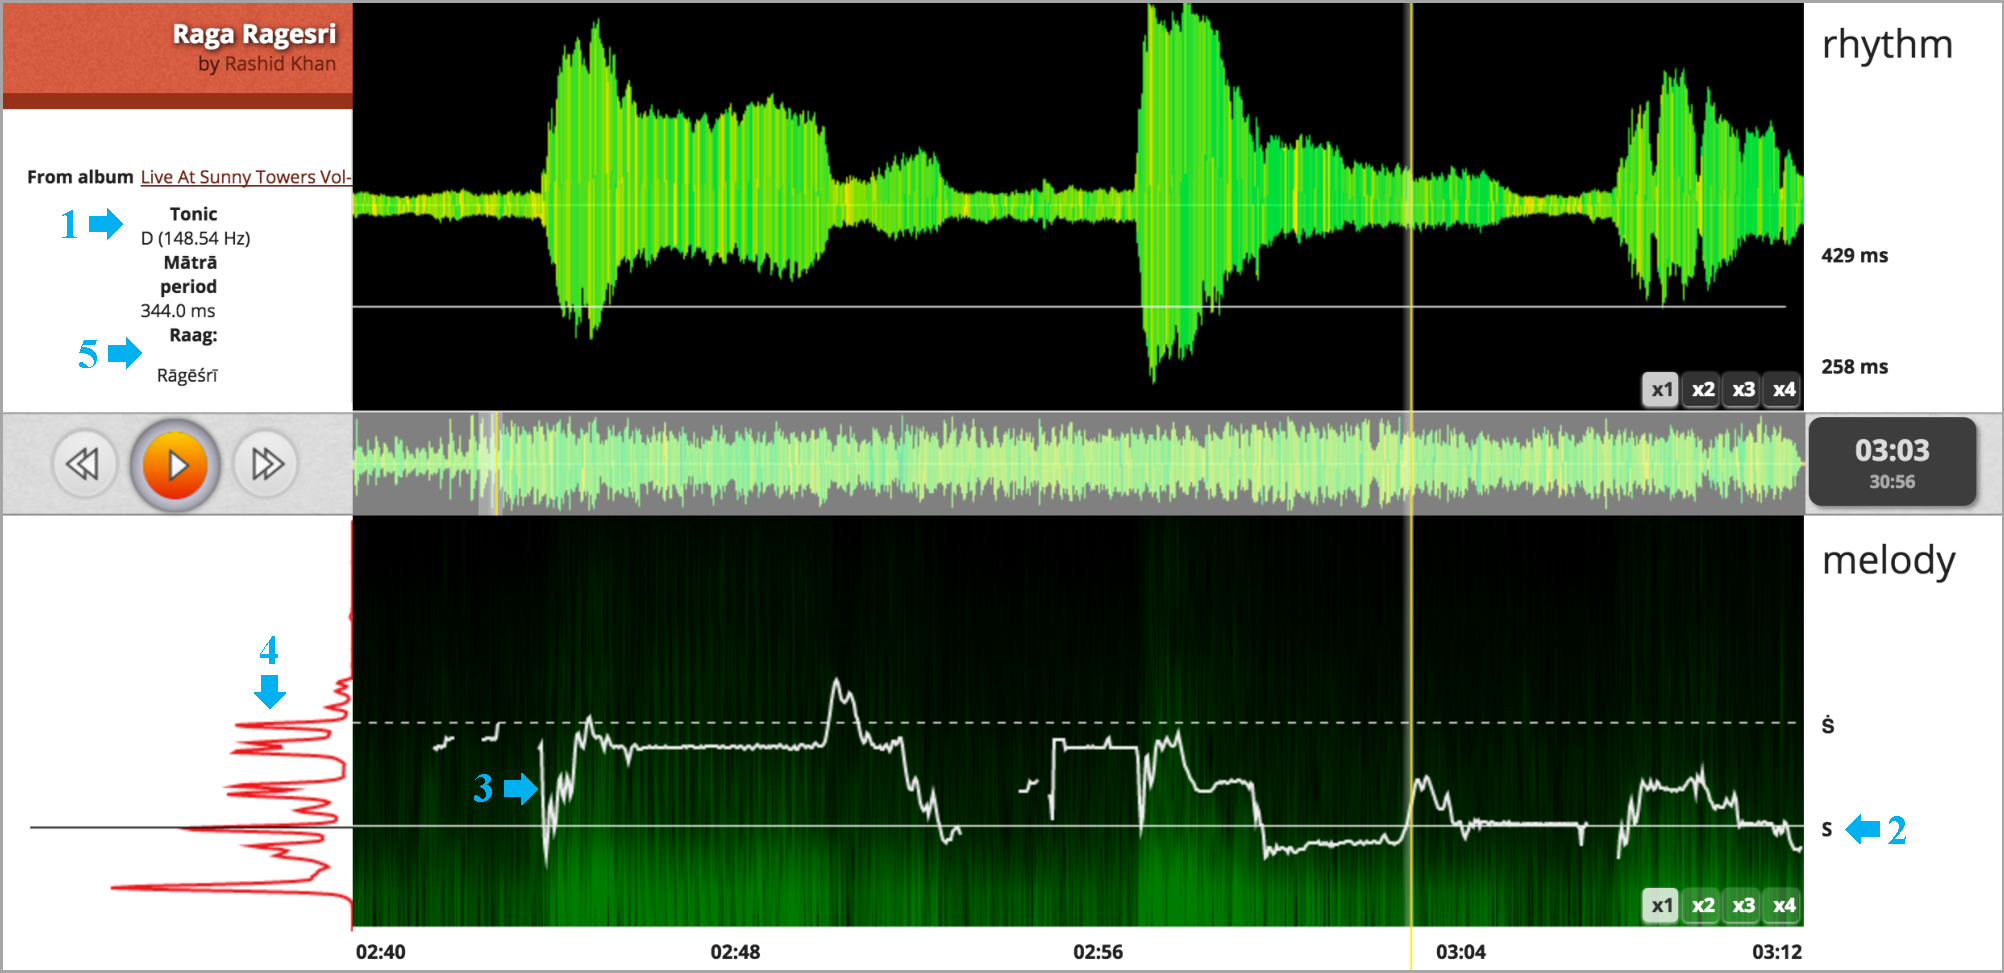
\includegraphics[width=\figSizeHundred]{ch08_applications/figures/dunyaScreenshot.pdf}
		\end{center}
		\caption{Screenshot of a recording page in Dunya showing showing extracted audio descriptors and relevant editorial metadata. Tonic, pitch histogram and melody is marked by XXX.}
		\label{fig:dunya_recording}
\end{sidewaysfigure}


\section{Mobile Applications: Sar\={a}ga and Riy\={a}z}
\label{sec:mobile_apps_camut}

\subsubsection{Sar\={a}ga}
\label{sec:saraga}



\begin{figure}
\centering
			\begin{subfigure}[b]{0.48\textwidth}
				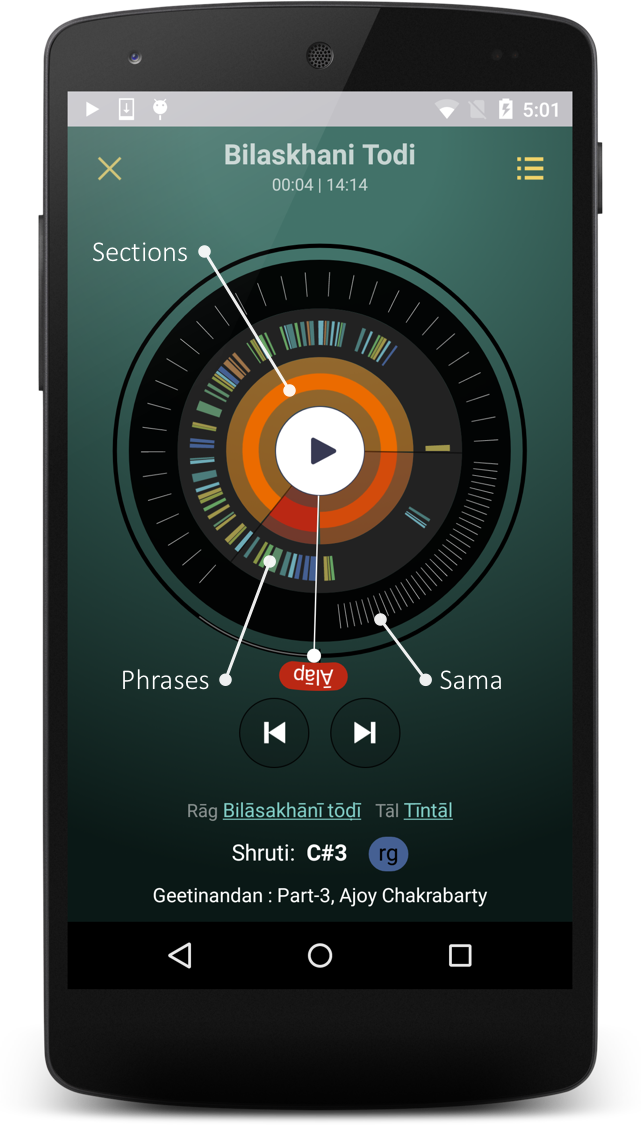
\includegraphics[width=\textwidth]{ch08_applications/figures/saraga1.png}
				\caption{Full music piece}
				\label{fig:saraga_full_piece}
			\end{subfigure}
			\begin{subfigure}[b]{0.48\textwidth}
				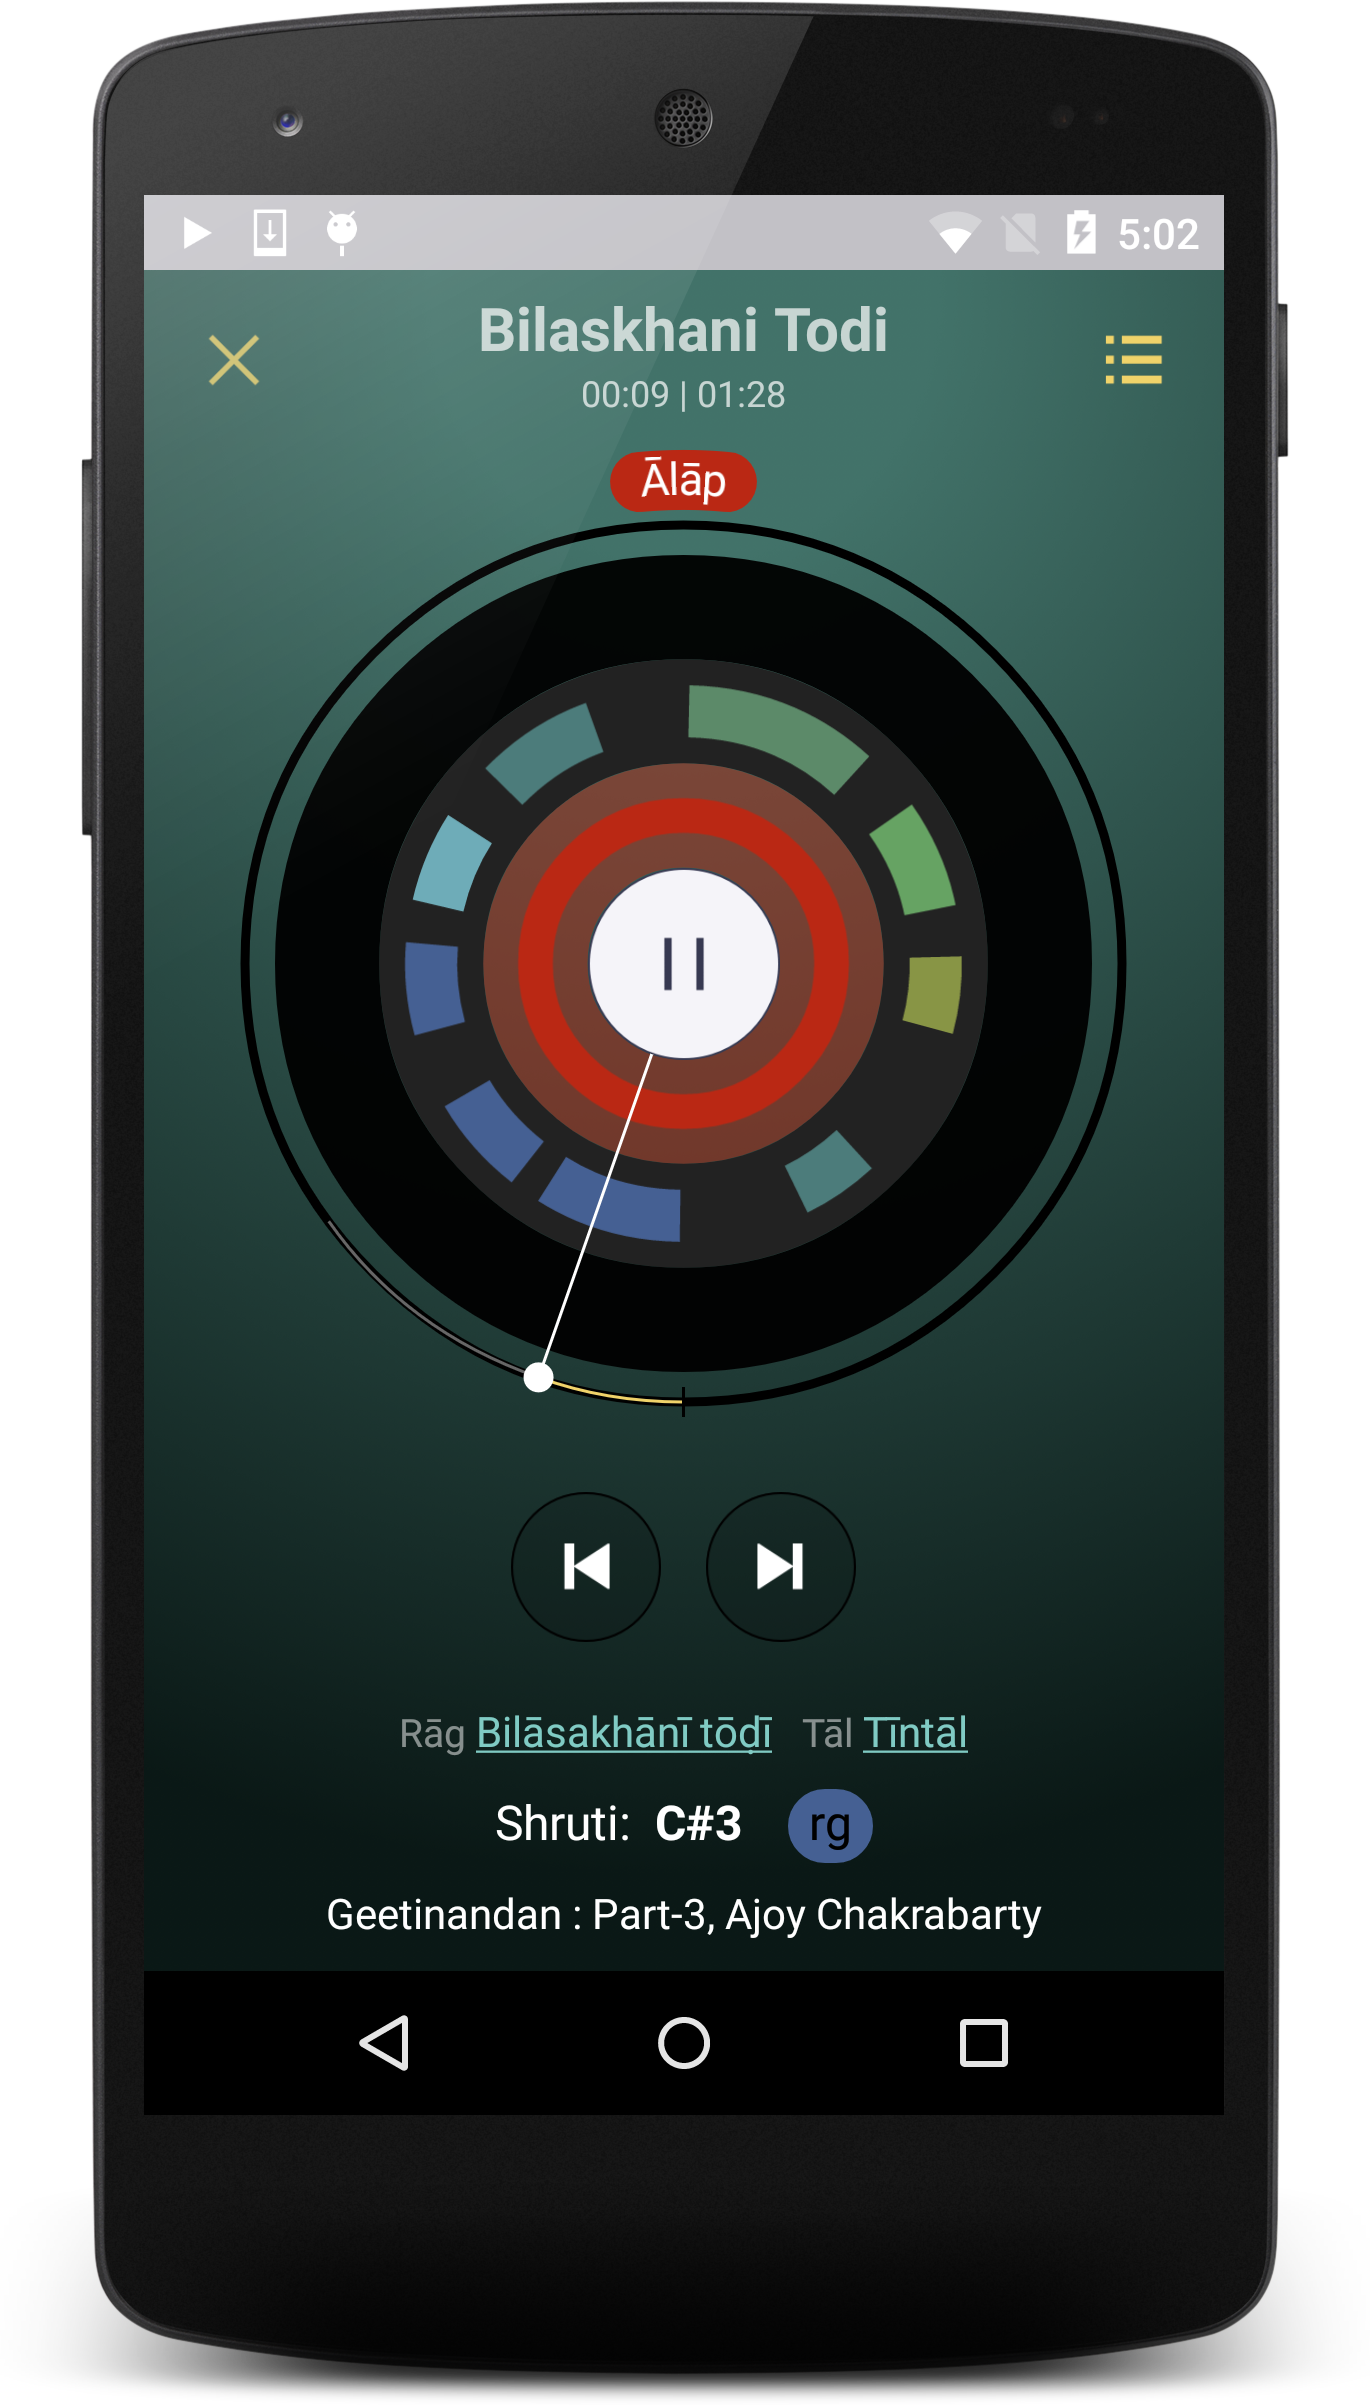
\includegraphics[width=\textwidth]{ch08_applications/figures/saraga2.png}
				\caption{\Gls{alap} section (zoomed in)}
				\label{fig:saraga_alap_section}
			\end{subfigure}
	\caption{Screenshots of Sar\={a}ga mobile application showing a music piece of Hindustani music. (a) shows the entire music piece, (b) shows the \gls{alap} section in the piece. The melodic phrases are marked by colored arches. Tonic (\gls{shruti}) of the recording is shown at the bottom along with the current playing melodic phrase.}
	\label{fig:saraga_screens}
\end{figure}



\subsubsection{Riy\={a}z}
\label{sec:riyaz}

\begin{figure}
	\begin{center}
		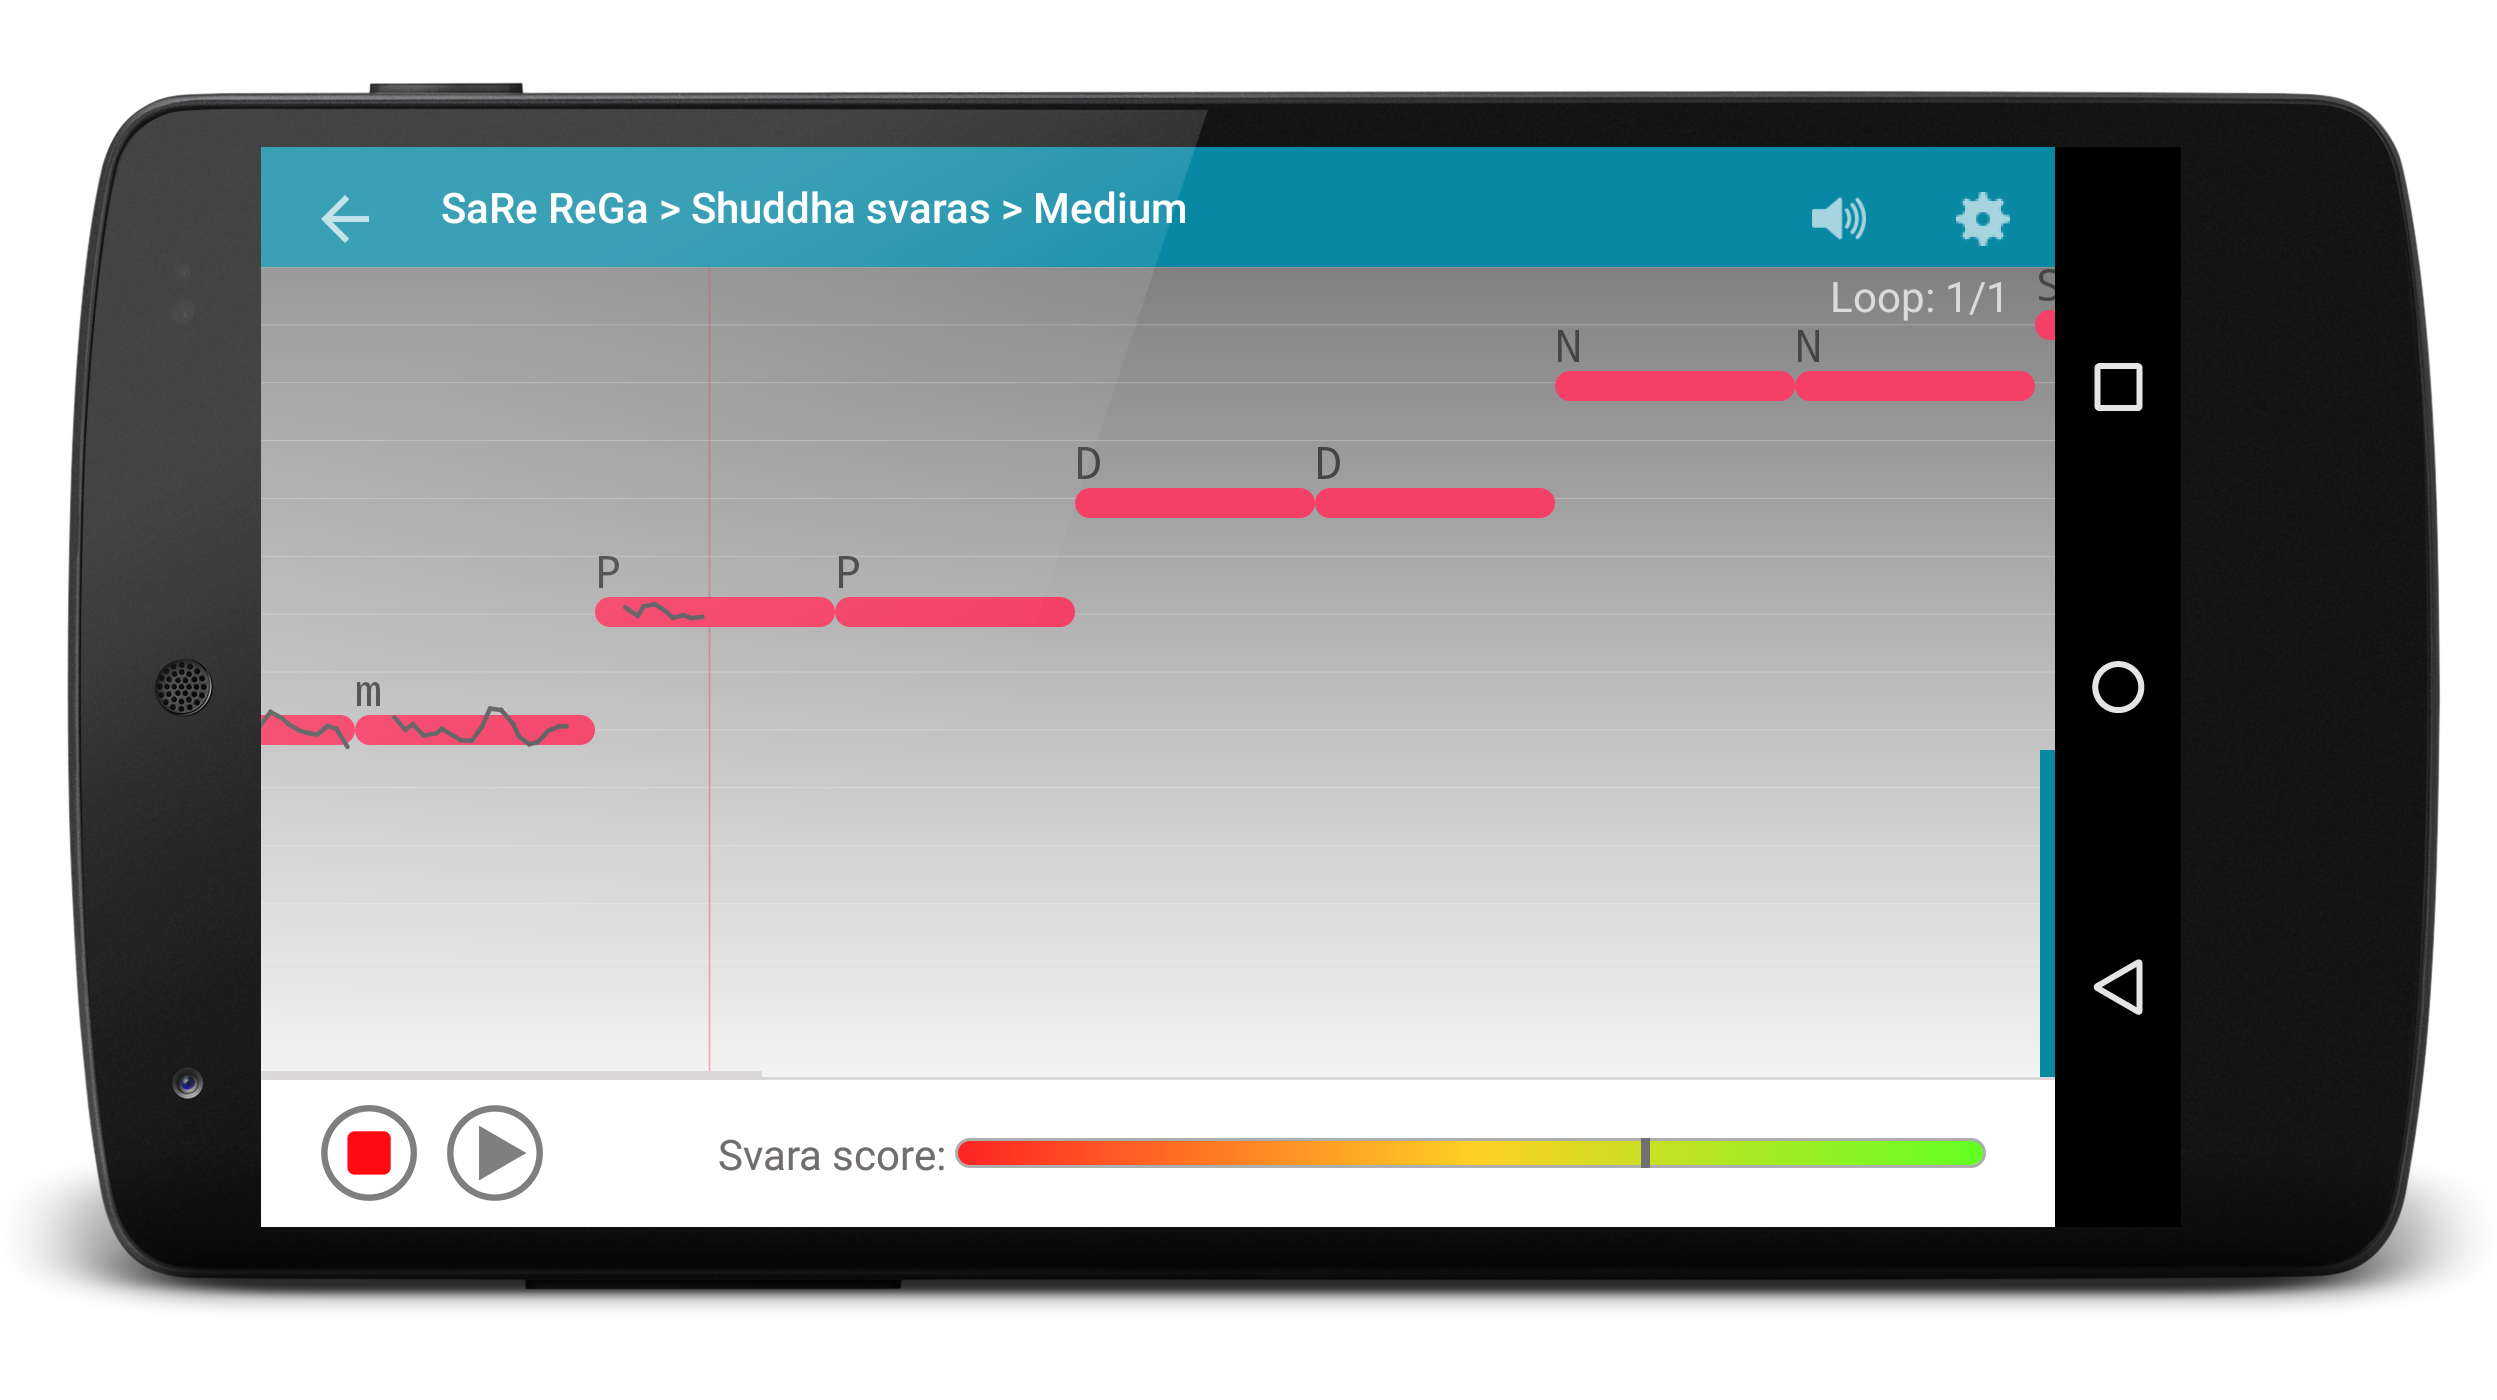
\includegraphics[width=\figSizeEightyFive]{ch08_applications/figures/riyaz1.png}
	\end{center}
	\caption{Screenshot of the evaluation screen in Riy\={a}z (Beta) mobile application showing real time melody extraction and scoring.}
	\label{fig:browser_patterns}
\end{figure}
\begin{figure}
	\begin{center}
		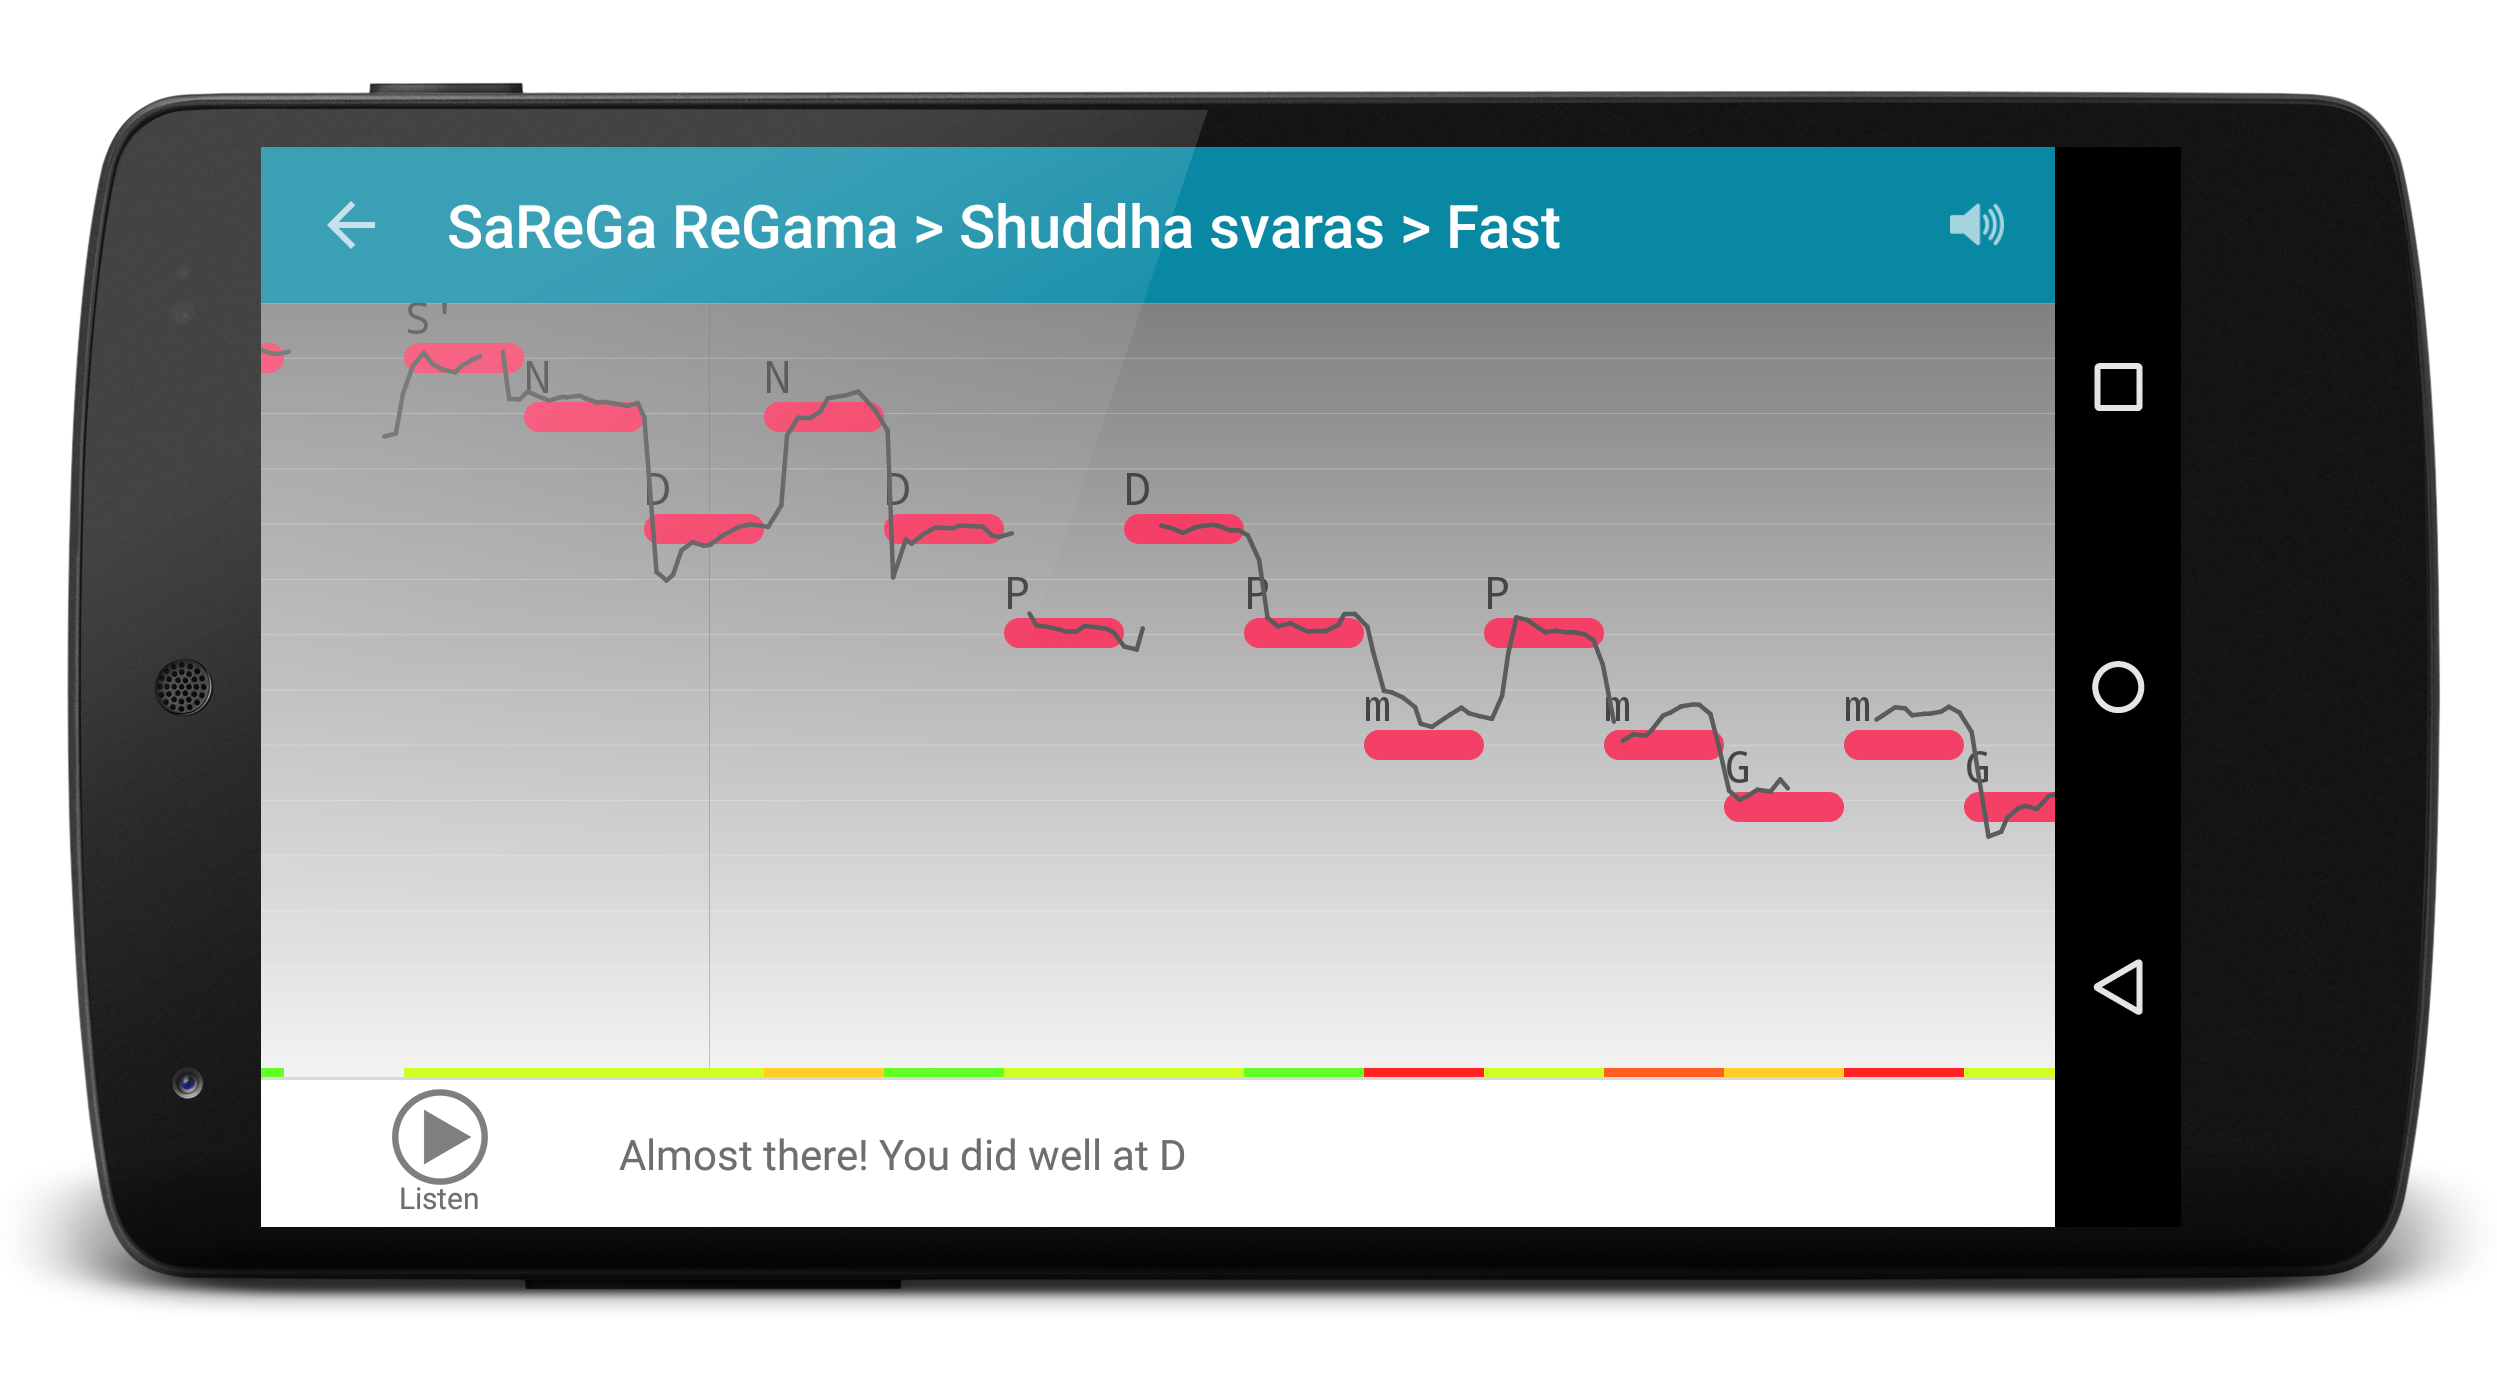
\includegraphics[width=\figSizeEightyFive]{ch08_applications/figures/riyaz2.png}
	\end{center}
	\caption{Screenshot of the feedback screen in Riy\={a}z (Beta) mobile application showing detailed feedback}
	\label{fig:browser_patterns}
\end{figure}


\section{Demos}
\subsection*{Demo1: Melodic Phrase-based Navigation of Collection}

\begin{figure}
	\begin{center}
		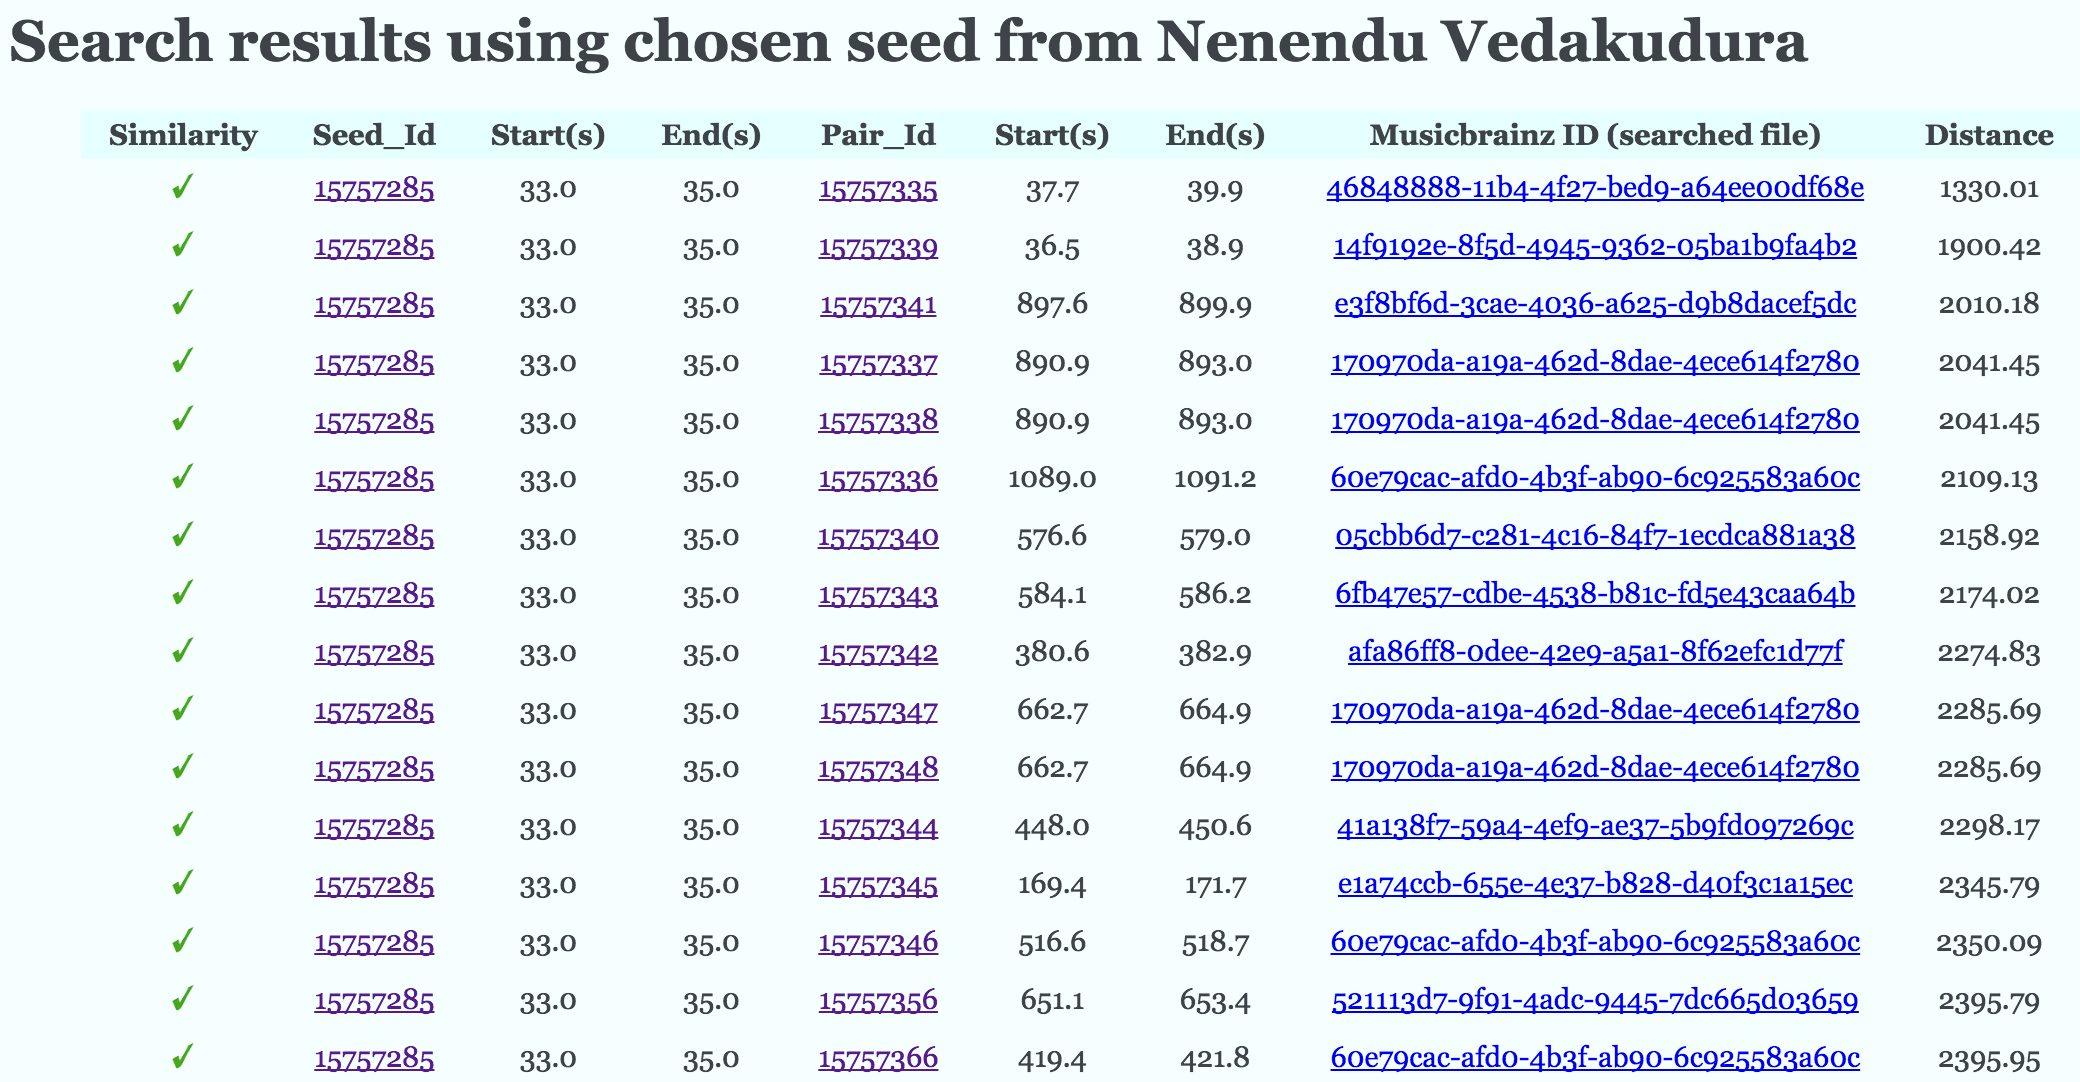
\includegraphics[width=\figSizeHundred]{ch08_applications/figures/patternBrowsing1.png}
	\end{center}
	\caption{Screenshot of a Web demo for navigating through the discovered melodic patterns organized by artists, releases and recordings.}
	\label{fig:browser_patterns}
\end{figure}

\subsection*{Demo2: Melodic Phrase-based Similarity Spaces}

\begin{figure}
	\begin{center}
		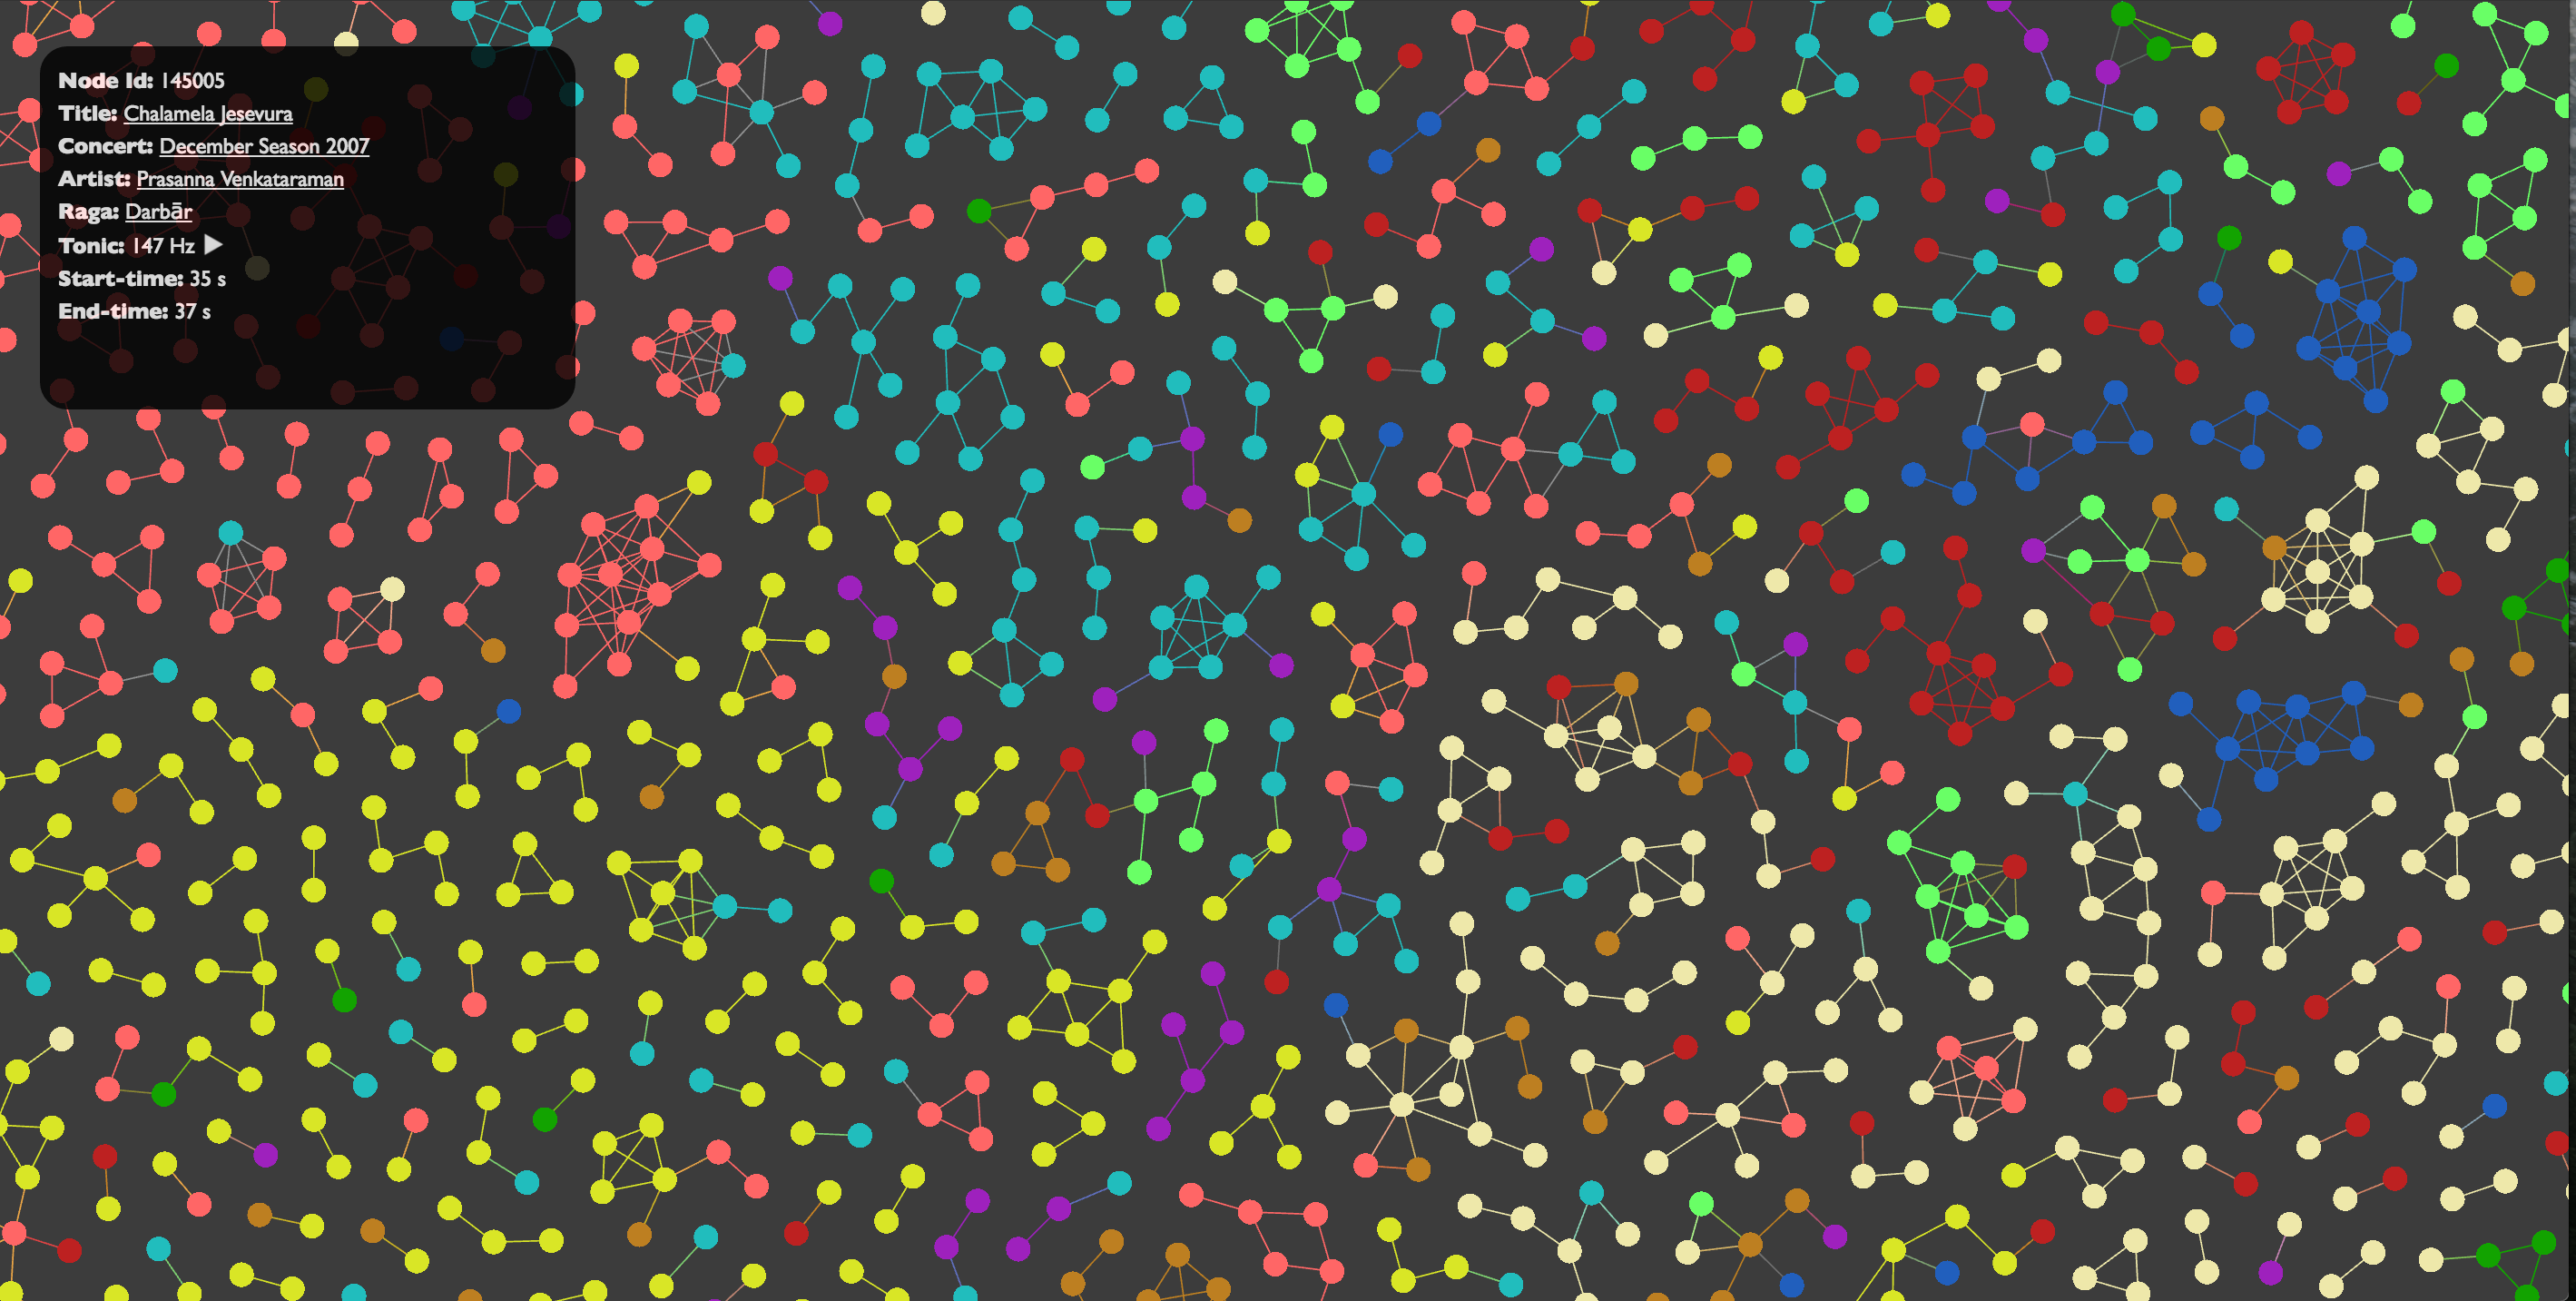
\includegraphics[width=\figSizeHundred]{ch08_applications/figures/patternNetwork1.png}
	\end{center}
	\caption{Screenshot of a Web demo of a network of the discovered melodic patterns. Colors indicate different \glspl{raga}.}
	\label{fig:network_patterns}
\end{figure}



\subsection{Ragawise: Realtime Raga Recognition}
\label{sec:ragawise}

\begin{sidewaysfigure}
	\begin{center}
		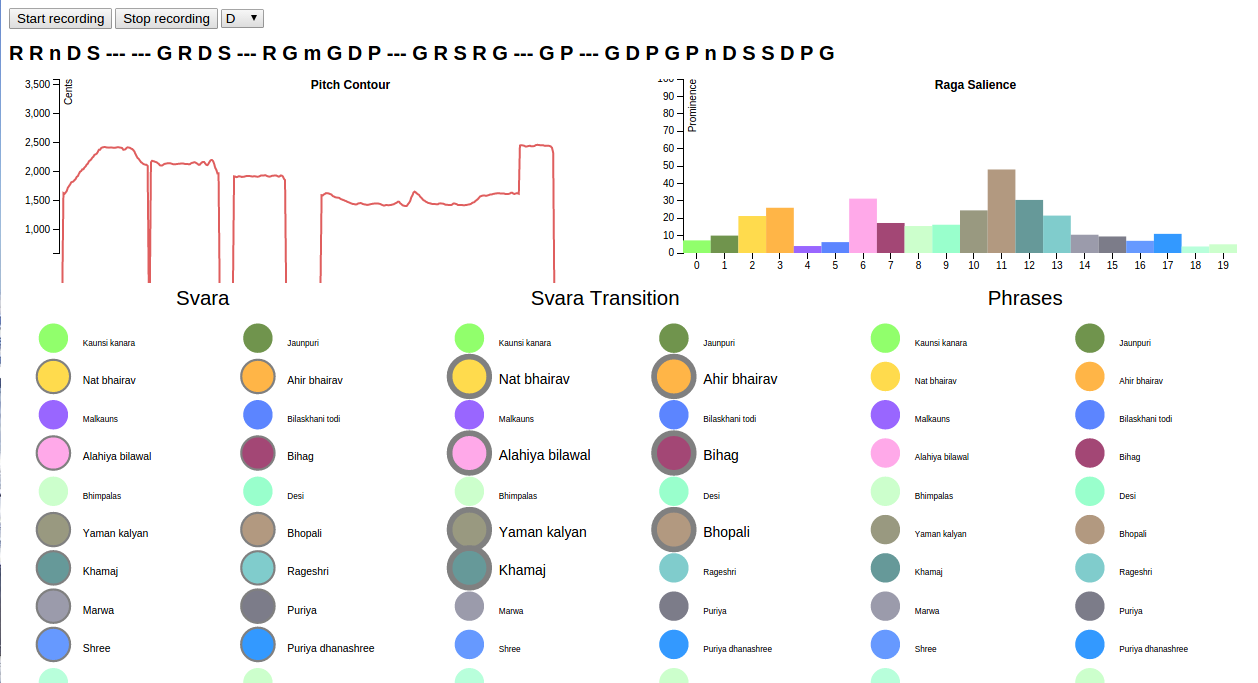
\includegraphics[width=\figSizeHundred]{ch08_applications/figures/ragawise.png}
	\end{center}
	\caption{Screenshot of Ragawisea recording page in Dunya showing showing extracted audio descriptors and relevant editorial metadata. Tonic, pitch histogram and melody is marked by XXX.}
	\label{fig:dunya_recording}
\end{sidewaysfigure}


\section{Tools for Musicological Studies}
\COMMENT{Write this section if you get time at the end}

\section{Summary}



